\documentclass[aspectratio=169]{beamer}
\usepackage[T1]{fontenc}
\usepackage[utf8]{inputenc}
\usepackage{tikz}
\usepackage{listings}
\usepackage{graphicx}
\usepackage{xcolor}

\usetheme{Madrid}
\usecolortheme{default}

% Code listing style
\lstset{
    basicstyle=\ttfamily\footnotesize,
    keywordstyle=\color{blue}\bfseries,
    commentstyle=\color{gray},
    stringstyle=\color{red},
    showstringspaces=false,
    breaklines=true,
    frame=single,
    language=Java
}

\title[Week 09: Game Loop \& Singleton]{Week 09: Design Patterns in Game Development}
\subtitle{Game Loop Pattern \& Singleton Pattern}
\author{Object-Oriented Programming Course}
\institute{Dungeon Escape: Progressive Learning}
\date{\today}

\begin{document}

%----------------------------------------------------------------------------------------
% TITLE SLIDE
%----------------------------------------------------------------------------------------

\begin{frame}
    \titlepage
\end{frame}

%----------------------------------------------------------------------------------------
% TABLE OF CONTENTS
%----------------------------------------------------------------------------------------

\begin{frame}{Outline}
    \tableofcontents
\end{frame}

%----------------------------------------------------------------------------------------
% SECTION 1: INTRODUCTION
%----------------------------------------------------------------------------------------

\section{Introduction}

\begin{frame}{Week 09 Overview}
    \begin{block}{Learning Objectives}
        \begin{itemize}
            \item Understand the \textbf{Game Loop Pattern}
            \item Learn separation of update and rendering
            \item Identify the \textbf{Object Drilling} anti-pattern
            \item Implement the \textbf{Singleton Pattern}
            \item Compare architectural trade-offs
        \end{itemize}
    \end{block}

    \vspace{0.5cm}

    \begin{block}{Progressive Branches}
        \begin{itemize}
            \item \texttt{09-00}: Monolithic design (the problem)
            \item \texttt{09-01}: Game Loop pattern (first solution)
            \item \texttt{09-02}: Without Singleton (new problem)
            \item \texttt{09-03}: With Singleton (final solution)
        \end{itemize}
    \end{block}
\end{frame}

%----------------------------------------------------------------------------------------
% SECTION 2: BRANCH 09-00
%----------------------------------------------------------------------------------------

\section{Branch 09-00: The Problem}

\begin{frame}{Branch 09-00: Monolithic Design}
    \begin{columns}[T]
        \begin{column}{0.5\textwidth}
            \textbf{What is it?}
            \begin{itemize}
                \item All code in one giant \texttt{main()} method
                \item 150+ lines in single method
                \item Update logic mixed with rendering
                \item No separation of concerns
            \end{itemize}

            \vspace{0.3cm}

            \textbf{Problems Demonstrated:}
            \begin{itemize}
                \item Frame rate coupling
                \item Untestable code
                \item Poor maintainability
                \item No scalability
            \end{itemize}
        \end{column}

        \begin{column}{0.5\textwidth}
            \textbf{Key Issue:}
            \begin{alertblock}{Frame Rate Coupling}
                Rendering delays slow down game logic by 80\%!
                \begin{itemize}
                    \item Render takes 50ms (flickering)
                    \item Only 2 FPS achieved
                    \item Game logic blocked by rendering
                \end{itemize}
            \end{alertblock}
        \end{column}
    \end{columns}
\end{frame}

\begin{frame}[fragile]{Branch 09-00: Code Structure}
    \begin{lstlisting}
public class Main {
    public static void main(String[] args) {
        // Initialize
        NPC npc = new NPC();
        Coin coin = new Coin();

        while (running) {
            // Update logic
            npc.move();
            coin.fall();
            checkCollisions();

            // Render (SLOW - causes problems!)
            clearScreen();
            draw(npc);
            draw(coin);
            Thread.sleep(50); // Flickering!
        }
    }
}
    \end{lstlisting}
\end{frame}

\begin{frame}{Branch 09-00: Performance Impact}
    \centering
    \textbf{Performance Metrics}

    \vspace{0.5cm}

    \begin{tabular}{|l|r|}
        \hline
        \textbf{Metric} & \textbf{Value} \\
        \hline
        Lines of Code (Main.java) & 150+ \\
        Frames Per Second & 2 FPS \\
        Testability & 0\% \\
        Maintainability & Very Low \\
        \hline
    \end{tabular}

    \vspace{0.5cm}

    \begin{alertblock}{Critical Issue}
        Cannot unit test logic without triggering rendering!
    \end{alertblock}
\end{frame}

%----------------------------------------------------------------------------------------
% SECTION 3: BRANCH 09-01
%----------------------------------------------------------------------------------------

\section{Branch 09-01: Game Loop Solution}

\begin{frame}{Branch 09-01: Game Loop Pattern}
    \begin{block}{Solution: Separation of Concerns}
        Split monolithic code into specialized classes:
        \begin{itemize}
            \item \texttt{GameEngine}: Controls the game loop
            \item \texttt{GameLogic}: Updates game state
            \item \texttt{GridRenderer}: Handles rendering only
        \end{itemize}
    \end{block}

    \vspace{0.3cm}

    \begin{columns}[T]
        \begin{column}{0.5\textwidth}
            \textbf{Key Concepts:}
            \begin{itemize}
                \item \texttt{update()} - Logic only
                \item \texttt{draw()} - Rendering only
                \item Delta time ($\Delta t$)
                \item Frame rate independence
            \end{itemize}
        \end{column}

        \begin{column}{0.5\textwidth}
            \textbf{Benefits:}
            \begin{itemize}
                \item Testable (no display needed)
                \item 60 FPS performance
                \item Clean separation
                \item Predictable behavior
            \end{itemize}
        \end{column}
    \end{columns}
\end{frame}

\begin{frame}[fragile]{Branch 09-01: Game Loop Structure}
    \begin{lstlisting}
public class GameEngine {
    private GameLogic logic;
    private boolean running = true;

    public void start() {
        while (running) {
            float delta = calculateDeltaTime();

            update(delta);  // Logic only
            draw();         // Render only
            sync();         // Control FPS (60 target)
        }
    }
}
    \end{lstlisting}
\end{frame}

\begin{frame}{Branch 09-01: Game Loop Flow Diagram}
    \centering
    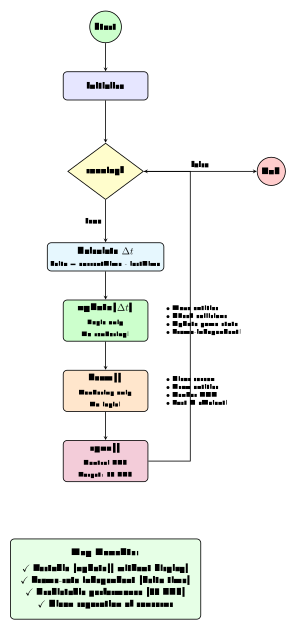
\includegraphics[width=0.8\textwidth]{../diagrams/game-loop-pattern.pdf}
\end{frame}

\begin{frame}{Branch 09-01: Performance Improvement}
    \centering
    \textbf{09-00 vs 09-01 Comparison}

    \vspace{0.5cm}

    \begin{tabular}{|l|r|r|c|}
        \hline
        \textbf{Metric} & \textbf{09-00} & \textbf{09-01} & \textbf{Change} \\
        \hline
        Lines in Main & 150+ & 3 & \textcolor{green}{50x reduction} \\
        FPS & 2 & 60 & \textcolor{green}{30x improvement} \\
        Testability & 0\% & 100\% & \textcolor{green}{Perfect} \\
        Flickering & Yes & No & \textcolor{green}{Fixed} \\
        \hline
    \end{tabular}

    \vspace{0.5cm}

    \begin{exampleblock}{Achievement Unlocked}
        Clean, testable, professional 60 FPS architecture!
    \end{exampleblock}
\end{frame}

%----------------------------------------------------------------------------------------
% SECTION 4: BRANCH 09-02
%----------------------------------------------------------------------------------------

\section{Branch 09-02: New Challenges}

\begin{frame}{Branch 09-02: Expanding the Game}
    \begin{block}{New Requirement}
        Add a HUD (Heads-Up Display) to show:
        \begin{itemize}
            \item Current score
            \item Game time
            \item Player level
        \end{itemize}
    \end{block}

    \vspace{0.3cm}

    \begin{alertblock}{Design Challenge}
        Multiple classes need to access the \texttt{GameManager}:
        \begin{itemize}
            \item \texttt{GameLogic} needs it to update score
            \item \texttt{HUD} needs it to display score
            \item \texttt{NPC} needs it to check game state
            \item \texttt{Coin} needs it to add points
        \end{itemize}
    \end{alertblock}
\end{frame}

\begin{frame}{Branch 09-02: Object Drilling Problem}
    \begin{columns}[T]
        \begin{column}{0.5\textwidth}
            \textbf{The Anti-Pattern:}
            \begin{itemize}
                \item Pass \texttt{manager} through constructors
                \item 4 levels deep!
                \item \texttt{Main} $\to$ \texttt{Engine} $\to$ \texttt{Logic} $\to$ \texttt{NPC}
                \item Every class polluted with parameters
            \end{itemize}

            \vspace{0.3cm}

            \textbf{Consequences:}
            \begin{itemize}
                \item 6+ files affected by changes
                \item Team collaboration conflicts
                \item Refactoring nightmare
                \item Constructor pollution
            \end{itemize}
        \end{column}

        \begin{column}{0.5\textwidth}
            \begin{alertblock}{Critical Bug!}
                \texttt{HUD} creates its own \texttt{GameManager} instance instead of using the shared one!

                \vspace{0.2cm}

                Result:
                \begin{itemize}
                    \item Score updates in instance A
                    \item HUD displays from instance B
                    \item Score shows 0 forever!
                \end{itemize}
            \end{alertblock}
        \end{column}
    \end{columns}
\end{frame}

\begin{frame}{Branch 09-02: Object Drilling Visualization}
    \centering
    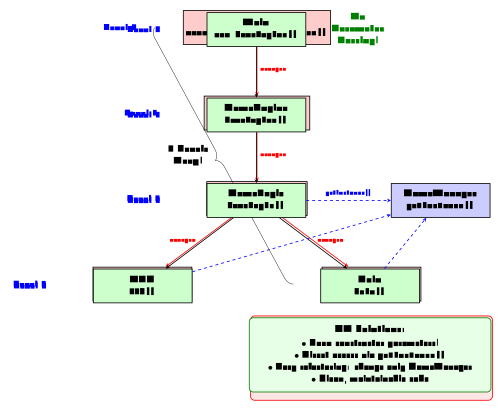
\includegraphics[width=0.9\textwidth]{../diagrams/object-drilling.pdf}
\end{frame}

\begin{frame}[fragile]{Branch 09-02: The Bug}
    \begin{lstlisting}
public class HUD {
    // BUG: Creates NEW instance!
    private final GameManager manager = new GameManager();

    public HUD(GameManager passedManager) {
        // Intentionally ignore the parameter!
        System.out.println("Using own instance!");
    }

    public void draw() {
        // Reads from WRONG instance!
        int score = manager.getScore();  // Always 0!
        System.out.println("Score: " + score);
    }
}
    \end{lstlisting}

    \begin{alertblock}{Output}
        \texttt{[GameManager:498931366] Score updated: 10}\\
        \texttt{[HUD] Score: 0}
    \end{alertblock}
\end{frame}

%----------------------------------------------------------------------------------------
% SECTION 5: BRANCH 09-03
%----------------------------------------------------------------------------------------

\section{Branch 09-03: Singleton Solution}

\begin{frame}{Branch 09-03: Singleton Pattern}
    \begin{block}{Solution: Guarantee Single Instance}
        The Singleton pattern ensures a class has only ONE instance and provides global access to it.
    \end{block}

    \vspace{0.3cm}

    \begin{columns}[T]
        \begin{column}{0.5\textwidth}
            \textbf{Three Key Components:}
            \begin{enumerate}
                \item Private static instance
                \item Private constructor
                \item Public static getInstance()
            \end{enumerate}
        \end{column}

        \begin{column}{0.5\textwidth}
            \textbf{Benefits:}
            \begin{itemize}
                \item Zero constructor parameters
                \item Guaranteed single instance
                \item Global access point
                \item Easy refactoring
            \end{itemize}
        \end{column}
    \end{columns}
\end{frame}

\begin{frame}{Branch 09-03: Singleton Pattern Diagram}
    \centering
    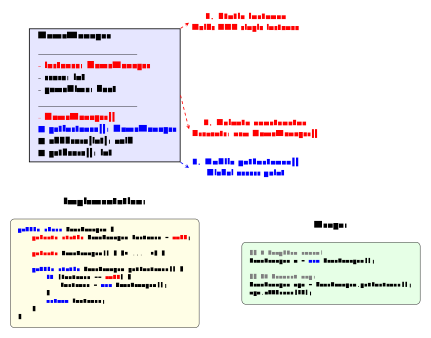
\includegraphics[width=0.7\textwidth]{../diagrams/singleton-pattern.pdf}
\end{frame}

\begin{frame}[fragile]{Branch 09-03: Implementation}
    \begin{lstlisting}
public class GameManager {
    // 1. Static instance (lazy initialization)
    private static GameManager instance = null;

    // 2. Private constructor (prevents: new GameManager())
    private GameManager() {
        this.score = 0;
        this.gameTime = 0.0f;
        this.level = 1;
    }

    // 3. Global access point
    public static GameManager getInstance() {
        if (instance == null) {
            instance = new GameManager();
        }
        return instance;
    }
}
    \end{lstlisting}
\end{frame}

\begin{frame}[fragile]{Branch 09-03: Clean Usage}
    \begin{lstlisting}
// Main.java - No parameters!
public class Main {
    public static void main(String[] args) {
        GameEngine engine = new GameEngine();
        engine.start();
    }
}

// HUD.java - Direct access!
public class HUD {
    public HUD() {
        // No parameters needed!
    }

    public void draw() {
        // Guaranteed to be THE instance
        int score = GameManager.getInstance().getScore();
        System.out.println("Score: " + score);
    }
}
    \end{lstlisting}
\end{frame}

%----------------------------------------------------------------------------------------
% SECTION 6: COMPARATIVE ANALYSIS
%----------------------------------------------------------------------------------------

\section{Comparative Analysis}

\begin{frame}{Architecture Evolution}
    \centering
    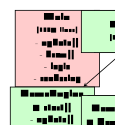
\includegraphics[width=0.95\textwidth]{../diagrams/uml-comparison.pdf}
\end{frame}

\begin{frame}{Performance Comparison}
    \centering
    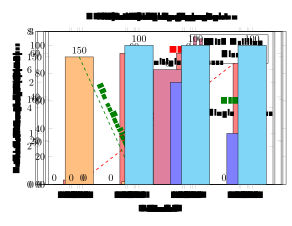
\includegraphics[width=0.85\textwidth]{../diagrams/performance-comparison.pdf}
\end{frame}

\begin{frame}{Comprehensive Metrics}
    \centering
    \begin{tabular}{|l|c|c|c|c|}
        \hline
        \textbf{Metric} & \textbf{09-00} & \textbf{09-01} & \textbf{09-02} & \textbf{09-03} \\
        \hline
        Lines in Main & 150+ & 3 & 32 & 3 \\
        FPS & 2 & 60 & 60 & 60 \\
        Testability & 0\% & 100\% & 100\% & 100\% \\
        Constructor Params & 0 & 0 & 6 & 0 \\
        GameManager Instances & 0 & 0 & 2 (BUG) & 1 \\
        Object Drilling Depth & N/A & N/A & 4 levels & 0 \\
        \hline
    \end{tabular}

    \vspace{0.5cm}

    \begin{exampleblock}{Final Achievement}
        Clean architecture with 60 FPS, zero object drilling, and guaranteed single instance!
    \end{exampleblock}
\end{frame}

%----------------------------------------------------------------------------------------
% SECTION 7: DESIGN PATTERNS DEEP DIVE
%----------------------------------------------------------------------------------------

\section{Design Patterns Deep Dive}

\begin{frame}{Game Loop Pattern}
    \begin{block}{Intent}
        Decouple the progression of game time from user input and processor speed.
    \end{block}

    \begin{columns}[T]
        \begin{column}{0.5\textwidth}
            \textbf{Structure:}
            \begin{itemize}
                \item \texttt{update(deltaTime)}
                \item \texttt{draw()}
                \item \texttt{sync()}
            \end{itemize}

            \vspace{0.3cm}

            \textbf{Participants:}
            \begin{itemize}
                \item GameEngine
                \item GameLogic
                \item Renderer
            \end{itemize}
        \end{column}

        \begin{column}{0.5\textwidth}
            \textbf{Consequences:}

            Benefits:
            \begin{itemize}
                \item Frame-rate independence
                \item Testability
                \item Clear separation
            \end{itemize}

            Liabilities:
            \begin{itemize}
                \item More classes
                \item Initial complexity
            \end{itemize}
        \end{column}
    \end{columns}
\end{frame}

\begin{frame}{Singleton Pattern}
    \begin{block}{Intent}
        Ensure a class has only one instance and provide a global point of access to it.
    \end{block}

    \begin{columns}[T]
        \begin{column}{0.5\textwidth}
            \textbf{When to Use:}
            \begin{itemize}
                \item Shared resource management
                \item Global state needed
                \item Exactly one instance required
            \end{itemize}

            \vspace{0.3cm}

            \textbf{Benefits:}
            \begin{itemize}
                \item Controlled access
                \item No global variables
                \item Lazy initialization
            \end{itemize}
        \end{column}

        \begin{column}{0.5\textwidth}
            \textbf{Liabilities:}
            \begin{itemize}
                \item Global state (testing harder)
                \item Hidden dependencies
                \item Thread safety concerns
            \end{itemize}

            \vspace{0.3cm}

            \textbf{Alternatives:}
            \begin{itemize}
                \item Dependency Injection
                \item Service Locator
                \item Static Class
            \end{itemize}
        \end{column}
    \end{columns}
\end{frame}

%----------------------------------------------------------------------------------------
% SECTION 8: CLASSROOM DISCUSSION
%----------------------------------------------------------------------------------------

\section{Discussion Points}

\begin{frame}{Discussion Questions}
    \textbf{For Students:}

    \begin{enumerate}
        \item Why is frame rate coupling a critical problem in games?
        \item What are the trade-offs of the Singleton pattern?
        \item When would you NOT use a Singleton?
        \item How does delta time enable frame-rate independence?
        \item What alternative to Singleton could we use?
    \end{enumerate}

    \vspace{0.5cm}

    \textbf{Critical Thinking:}
    \begin{itemize}
        \item Is global state always bad?
        \item How would you test a class that uses GameManager.getInstance()?
        \item What happens in a multi-threaded environment?
    \end{itemize}
\end{frame}

%----------------------------------------------------------------------------------------
% SECTION 9: ASSESSMENT
%----------------------------------------------------------------------------------------

\section{Assessment}

\begin{frame}{Assessment Rubric (100 points)}
    \begin{tabular}{|l|r|p{6cm}|}
        \hline
        \textbf{Component} & \textbf{Points} & \textbf{Criteria} \\
        \hline
        Code Implementation & 40 & Correct Singleton, working game loop \\
        Testing & 20 & Unit tests for GameLogic, coverage $>$ 80\% \\
        Design & 20 & UML diagrams, architecture explanation \\
        Documentation & 10 & JavaDoc, README, design decisions \\
        Code Quality & 10 & Style, no warnings, clean code \\
        \hline
        \textbf{Total} & \textbf{100} & \\
        \hline
    \end{tabular}
\end{frame}

%----------------------------------------------------------------------------------------
% SECTION 10: SUMMARY
%----------------------------------------------------------------------------------------

\section{Summary}

\begin{frame}{Week 09 Summary}
    \begin{block}{Key Takeaways}
        \begin{itemize}
            \item \textbf{Game Loop Pattern}: Separates update from rendering
            \item \textbf{Delta Time}: Enables frame-rate independence
            \item \textbf{Object Drilling}: Anti-pattern to avoid
            \item \textbf{Singleton Pattern}: Guarantees single instance
            \item \textbf{Trade-offs}: Every pattern has benefits and costs
        \end{itemize}
    \end{block}

    \vspace{0.3cm}

    \begin{block}{Progressive Learning Journey}
        \texttt{09-00} (Problem) $\to$ \texttt{09-01} (Solution) $\to$ \texttt{09-02} (New Problem) $\to$ \texttt{09-03} (Final Solution)
    \end{block}

    \vspace{0.3cm}

    \begin{exampleblock}{Result}
        Professional game architecture: 60 FPS, testable, maintainable, scalable!
    \end{exampleblock}
\end{frame}

%----------------------------------------------------------------------------------------
% CLOSING SLIDE
%----------------------------------------------------------------------------------------

\begin{frame}[plain,c]
    \begin{center}
        {\Huge Thank You!}

        \bigskip\bigskip

        {\LARGE Questions? Comments?}

        \vspace{1cm}

        \textit{Next Week: Observer Pattern \& Event Systems}
    \end{center}
\end{frame}

\end{document}
